\documentclass[11pt]{article}

\usepackage[margin=1in]{geometry}
\usepackage{amsmath, amssymb}
\usepackage{booktabs}
\usepackage{graphicx}
\usepackage{float}
\usepackage{hyperref}
\usepackage{subcaption}
\usepackage{xcolor}

\graphicspath{{figures/}}

\newcommand{\placeholder}[1]{%
  \par\noindent\textcolor{gray}{\fbox{\begin{minipage}{0.96\linewidth}
  \textbf{Placeholder:} #1
  \end{minipage}}}\par\vspace{0.75em}
}
\newcommand{\question}[1]{\subsection*{#1}}
\newcommand{\subquestion}[1]{\subsubsection*{#1}}
\newcommand{\figureplaceholder}[1]{%
  \fbox{\begin{minipage}[c][2.2in][c]{0.9\linewidth}
  \centering #1
  \end{minipage}}
}

\title{CS336 Assignment 2: Systems and Parallelism}
\author{Lenard Strahringer}
\date{\today}

\begin{document}
\maketitle

\section*{2 Profiling and Benchmarking}

\question{Problem: Benchmarking Script}
\subquestion{(a) Benchmarking script implementation}
Script: \texttt{benchmarking/benchmarking\_script.py}. 

\subquestion{(b) Model-size timing results}
Table \ref{benchmarking_script_results_1} presents the results of the benchmarking. 

\begin{table}[H]
  \centering
  \input{tables/benchmarking_script_results_1.tex}
  \caption{Mean and standard deviation of forward, backward, and optimizer-step timings in seconds on a Modal B200, using batch size 4, context length 256, 5 warm-up steps, 10 measurement steps, and bfloat16 weights.}
  \label{benchmarking_script_results_1}
\end{table}

The forward pass ranges from 0.011\,s for the small model to 0.284\,s for the 7B model. The backward pass ranges from 0.018\,s to 0.519\,s and is consistently more expensive than the forward pass. Standard deviations are small relative to the means for the forward pass. The largest models show somewhat more variability for backward and optimizer-step timing.

\subquestion{(c) Warm-up ablation}
With zero warm-up steps, the first measurement includes CUDA lazy context initialization, cuBLAS GEMM algorithm selection, and PyTorch allocator bookkeeping. These one-time costs make the first timing several times the steady-state value and produce large standard deviations. With 1--2 warm-up steps, CUDA is already initialized, and the allocator has committed the required memory, so most measurements drop close together. For larger models, the second or third step can still be slower because PyTorch's autograd JIT graph may not have fully converged, and cuBLAS can still be refining its GEMM kernel selection for the widest matrix dimensions. Five warm-up steps are sufficient to saturate all caches for every model size tested, which results in small standard deviations.

\question{Problem: Nsight Systems Profiling}
\subquestion{(a) Forward-pass time}
At batch size 4 on a Modal B200 (FP32 full training step), the small model fits up to context 4096 and the medium model fits up to context 2048; both OOM at the next power of two due to $O(T^2)$ attention matrices.

\begin{table}[H]
  \centering
  \input{tables/nsys_profile_forward_summary.tex}
  \caption{Forward-pass time from Nsight Systems CUDA GPU kernel summaries compared with the Python standard-library timing benchmark.}
  \label{tab:nsys-forward-summary}
\end{table}

Table~\ref{tab:nsys-forward-summary} shows that the Nsight forward-pass GPU kernel time agrees reasonably well with the Python benchmark. For example, the small model at context 4096 is 256.6\,ms in Nsight versus 294.9\,ms from Python, and the medium model at context 2048 is 252.9\,ms versus 274.0\,ms. The Python timing is slightly larger.

\subquestion{(b) Dominant CUDA kernel}
\begin{table}[H]
  \centering
  \resizebox{\textwidth}{!}{\input{tables/nsys_profile_kernel_summary.tex}}
  \caption{Dominant forward-pass kernel family and aggregate kernel fractions from Nsight Systems. ``FBO'' denotes the full forward, backward, and optimizer-step profile.}
  \label{tab:nsys-kernel-summary}
\end{table}

Table~\ref{tab:nsys-kernel-summary}: the dominant forward-pass CUDA kernel is a CUTLASS FP32 SGEMM kernel in every profiled configuration. The top kernel is invoked between 24 and 97 times depending on model size and context length. It is also the dominant kernel in the forward-plus-backward profiles for most settings, though at the small model with context 4096, an elementwise kernel becomes the largest kernel in the full training-step profile.

\subquestion{(c) Non-matmul kernels}
Besides matrix multiplies, the main non-trivial forward kernels are softmax-related and elementwise kernels: max reductions, exponentials, sum reductions, residual and normalization elementwise operations, SwiGLU sigmoid and elementwise kernels, and batched copy/cat kernels.

\subquestion{(d) Full training-step profile}
The matrix-multiplication fraction drops when moving from inference to a full training step. For example, small context 256 goes from 78.2\% to 64.7\%, medium context 256 goes from 81.0\% to 68.3\%, and medium context 2048 goes from 62.8\% to 61.2\%. Elementwise kernels become clearly more important in the full step, reaching 28--36\% in most configurations and 47.7\% for the small model at context 4096.

\subquestion{(e) Attention softmax versus matmul}
Softmax-related kernels are definitely cheaper than the matrix multiplies, but not by the same margin suggested by FLOP counts. For the small model at context 4096, matmul kernels take 49.8\% of forward GPU time while softmax-related kernels account for 10.1\%. For the medium model at context 2048, the split is 62.8\% versus 7.1\%. Softmax runtime is relatively high for its FLOP count because it requires a lot of memory traffic, reductions, and exponentials rather than GPU compute.

\question{Problem: Mixed-Precision Accumulation}
Script \texttt{precision\_accumulation.py} gives $10.0001$ for all-FP32 accumulation, $9.9531$ when both the accumulator and addends are FP16, and $10.0021$ when the accumulator is FP32 but each term is first written as FP16. The FP16 run loses almost half a unit because the half-precision accumulator has growing ULPs, so many later additions round away. The last two cases match because in-place addition into FP32 promotes the addend; the residual bias versus $10$ comes from FP16's coarse representation of $0.01$, not from the accumulator dtype.

\question{Problem: Benchmarking Mixed Precision}
\subquestion{(a) Autocast dtypes in ToyModel}
On a CUDA GPU with \texttt{torch.autocast(device\_type="cuda", dtype=torch.float16)} and FP32 parameters: stored weights remain FP32; the \texttt{fc1} (post-ReLU) activation is FP16; \texttt{LayerNorm} runs in full precision so its output is FP32; \texttt{fc2} logits are FP16; cross-entropy loss is evaluated in FP32; gradients w.r.t.\ the FP32 parameters are FP32.

\subquestion{(b) Layer normalization and mixed precision}
Reductions for the mean and variance are sensitive. Also, the estimation of centered second moments with a small variance. Division by $\sigma$ and the preceding \texttt{sqrt} amplify any error in $\mu$ and $\sigma^2$. BF16 shares FP32's exponent range, so extreme overflow and underflow are less of a concern than with FP16. However, BF16's 7-bit trailing mantissa means rounding in sums and cancellation can still matter.

\subquestion{(c) Transformer mixed-precision benchmarking}
\begin{table}[H]
  \centering
  % Auto-generated by cs336_systems/profiling_benchmarking/benchmarking_script_experiment_mixed_precision.py.
\begin{tabular}{lrrrrrrrr}
\toprule
Model & \multicolumn{2}{c}{Forward FP32} & \multicolumn{2}{c}{Forward BF16} & \multicolumn{2}{c}{Backward FP32} & \multicolumn{2}{c}{Backward BF16} \\
\cmidrule(lr){2-3} \cmidrule(lr){4-5} \cmidrule(lr){6-7} \cmidrule(lr){8-9}
 & mean (s) & sd & mean (s) & sd & mean (s) & sd & mean (s) & sd \\
\midrule
small & 0.010975 & 0.003595 & 0.007213 & 0.000023 & 0.018698 & 0.000384 & 0.014916 & 0.000340 \\
medium & 0.026192 & 0.005949 & 0.014165 & 0.000131 & 0.048544 & 0.000372 & 0.028838 & 0.000271 \\
large & 0.065349 & 0.010402 & 0.021287 & 0.000036 & 0.111151 & 0.002344 & 0.035236 & 0.000153 \\
xl & 0.165036 & 0.030192 & 0.025298 & 0.003149 & 0.299348 & 0.003768 & 0.063578 & 0.000492 \\
7B & 0.283873 & 0.051970 & 0.035896 & 0.004677 & 0.519411 & 0.005211 & 0.098109 & 0.002179 \\
\bottomrule
\end{tabular}

  \caption{Forward and backward timings on Modal B200, batch size 4, context length 256, $5$ warm-up and $10$ timed steps per configuration;}
  \label{tab:benchmark-mixed-precision}
\end{table}

Table~\ref{tab:benchmark-mixed-precision} presents the benchmarking results. BF16 lowers forward means by about $1.5\times$ on \emph{small}, about $3\times$ on \emph{large}, and about $6.5$--$8\times$ on \emph{xl} and \emph{7B}. Backward speedups are more muted, roughly $1.3\times$ up to $\sim5.3\times$. Timings also become much less variable under BF16 for the bigger models. For example, xl forward standard deviation falls from $0.030$\,s to $0.003$\,s.

\question{Problem: Memory Profiling}
\subquestion{(a) Active memory timelines}
Figure~\ref{fig:mem-xl-forward} shows the active memory timeline for an \emph{xl} forward-only step (context length $2048$, batch $4$, BF16 \texttt{autocast}). Figure~\ref{fig:mem-xl-fbo} shows a full training step (forward, backward, AdamW) with the same context and BF16 \texttt{autocast} on batch $2$, because batch $4$ at this configuration exceeds available memory. The forward-only trace is a roughly flat baseline ($\sim$13\,GiB) with periodic spikes up to $\sim$18.6\,GiB caused by the activations of the \texttt{TransformerBlock}s. The full-step trace shows a sizable increase from $\sim$37\,GiB to $\sim$112\,GiB through forward as residuals accrue, then a stepped descent through backward as those tensors are freed while gradients appear, with a small rise near the optimizer update.

\begin{figure}[H]
  \centering
  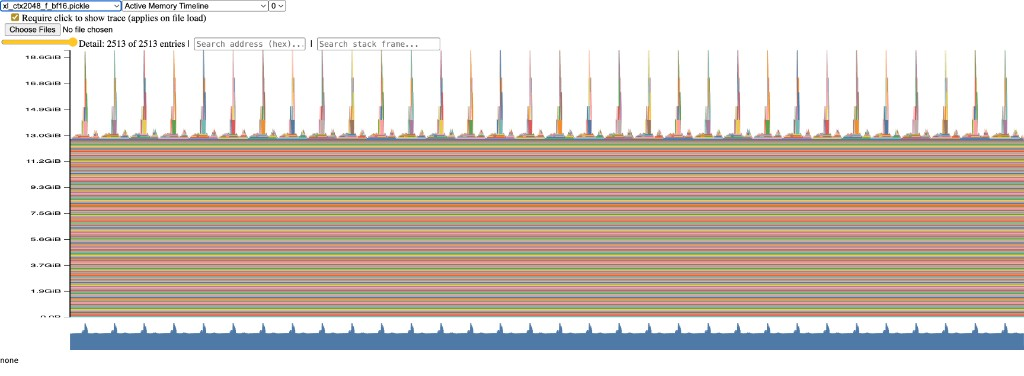
\includegraphics[width=\linewidth]{figures/memory_xl_ctx2048_forward_bf16.png}
  \caption{Active memory timeline: \emph{xl} inference-style forward (single step, \texttt{torch.inference\_mode}), context $2048$, batch $4$, BF16 \texttt{autocast}}
  \label{fig:mem-xl-forward}
\end{figure}

\begin{figure}[H]
  \centering
  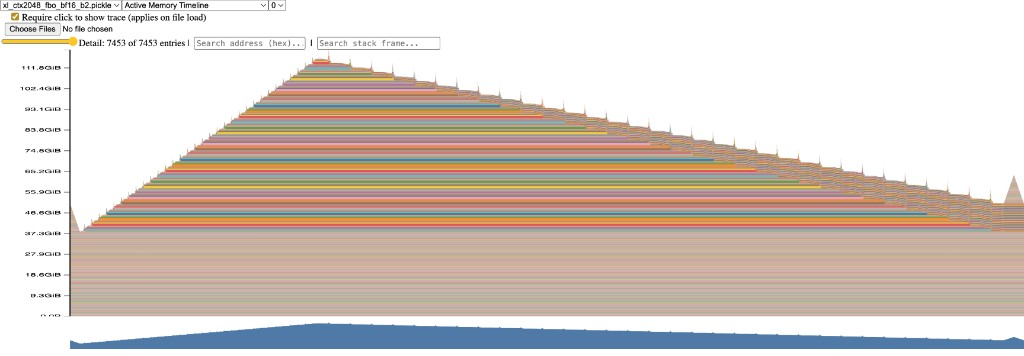
\includegraphics[width=\linewidth]{figures/memory_xl_ctx2048_fbo_bf16_b2.png}
  \caption{Active memory timeline: \emph{xl} full training step, context $2048$, batch $2$, BF16 \texttt{autocast}}
  \label{fig:mem-xl-fbo}
\end{figure}

\subquestion{(b) Peak memory by context length}
Peaks are CUDA \texttt{max\_memory\_allocated()} during the traced step (Modal B200). Numbers below use FP32 matmuls for comparability; full training at context $2048$ uses batch $2$ (see footnote in table).

\begin{table}[H]
  \centering
  \begin{tabular}{lrrr}
  \toprule
  Context & Step & Peak alloc.\ (GiB) & batch \\
  \midrule
  128 & Forward (FP32) & $12.78$ & 4 \\
  128 & Full training (FP32) & $63.49$ & 4 \\
  2048 & Forward (FP32) & $21.18$ & 4 \\
  2048 & Full training (FP32) & $143.43$ & 2$^*$ \\
  \bottomrule
\end{tabular}

  \caption{Peak allocated memory (\texttt{torch.cuda.max\_memory\_allocated}) for \emph{xl}}
  \label{tab:memory-peaks}
\end{table}

\smallskip\noindent$^*$Attention materializes large $[B, H, T, T]$ tensors; at $T{=}2048$, batch $4$ for a full step exceeds memory, so I changed to batch $2$.

\subquestion{(c) Mixed-precision peak memory}
At context $128$, BF16 \texttt{autocast} leaves peaks almost unchanged (forward $\approx 12.78$\,GiB FP32 vs.\ $\approx 12.79$\,GiB BF16; full step $\approx 63.49$\,GiB vs.\ $\approx 63.48$\,GiB). Memory at short context is dominated by FP32 weights, optimizer state, and other FP32 paths rather than activations. At context $2048$, forward peak drops from $\approx 21.18$\,GiB (FP32) to $\approx 19.14$\,GiB (BF16), and the full step at batch $2$ drops from $\approx 143.43$\,GiB to $\approx 119.98$\,GiB. Mixed precision reduces memory, and more so with long context, where dense attention and block activations make up for a large fraction of the peak.

\subquestion{(d) Residual-stream activation size}
The post-embedding hidden states entering each block have shape $[\text{batch}, \text{seq length}, d_{\text{model}}]$; in FP32 that is $4 \cdot B \cdot T \cdot d_{\text{model}}$ bytes. For \emph{xl} ($d_{\text{model}}{=}2560$) at batch $4$, this is $4 \times 4 \times T \times 2560 = 40{,}960\,T$ bytes. That is $5$\,MiB at $T{=}128$ and $80$\,MiB at $T{=}2048$ (using MiB${}=2^{20}$).

\subquestion{(e) Largest allocations in memory-viz}
The dominant blocks are on the order of $\sim$1\,GiB per-layer, matching FP32 tensors shaped like pre-softmax scores or attention weights $[B, n_{\text{heads}}, T, T]$ (e.g.\ $2 \times 32 \times 2048^2 \times 4$\,bytes $\approx 1$\,GiB at batch $2$). Stack traces point to the \texttt{einsum} computing $QK^\top$ and the \texttt{softmax} path that materializes the normalized weights.

\subquestion{(f) Per-block memory attribution}
Figure~\ref{fig:memory-viz-per-block} shows the active-memory timeline zoomed to the forward pass of the \emph{xl} model (batch 2, context 2048, FP32.

\begin{figure}[H]
  \centering
  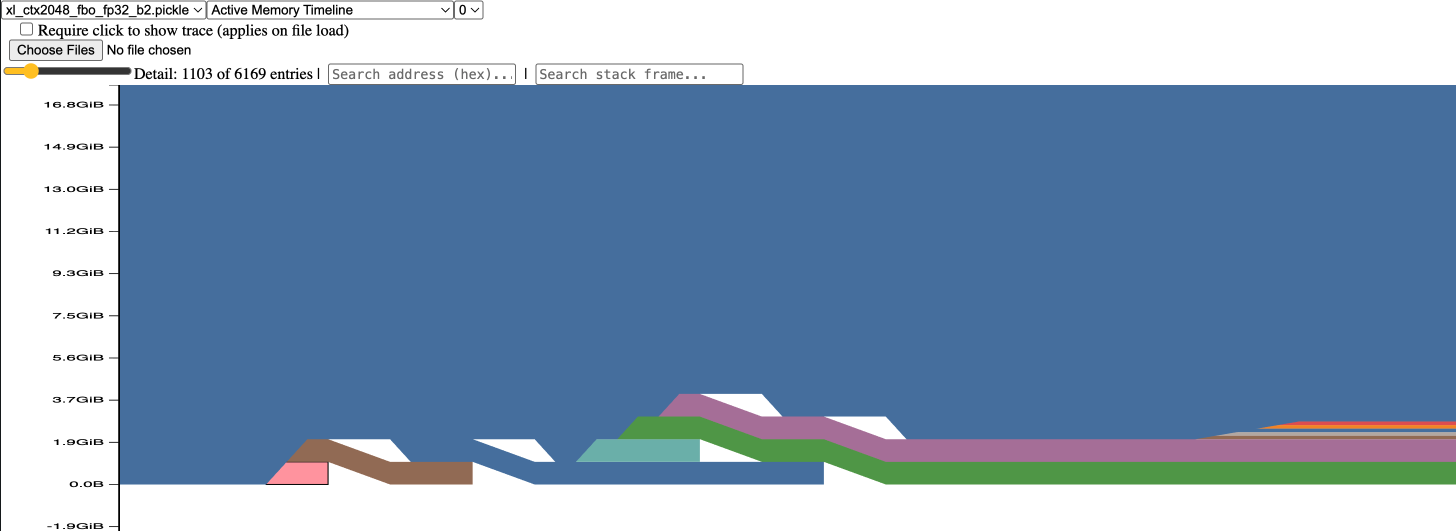
\includegraphics[width=\linewidth]{figures/memory_viz_per_block_annotated.png}
  \caption{Active-memory timeline zoomed to the forward pass (\emph{xl}, batch 2, ctx 2048, FP32). Each colored band is one large allocation; colors correspond to the legend in the text.}
  \label{fig:memory-viz-per-block}
\end{figure}

\paragraph{Attention tensors (each 1\,GiB, shape $[2,32,2048,2048]$ in FP32).}
Traces show six separate $[B,H,T,T]$ allocations per attention layer:
\begin{enumerate}
  \item Pink: $QK^\top$ --- output of \texttt{einsum} at \texttt{model.py:427}.
  \item Brown: $S=QK^\top/\sqrt{d}$ --- \texttt{div} at \texttt{model.py:427}.
  \item Blue (bottom): masked scores --- \texttt{where} (causal mask) at \texttt{model.py:430}.
  \item Light blue: $S-\max(S)$ --- \texttt{sub} at \texttt{nn\_utils.py:5} (numerical stability shift).
  \item Green: $\exp(S-\max)$ --- \texttt{exp} at \texttt{nn\_utils.py:6}.
  \item Purple: $P=\mathrm{softmax}(S)$ --- \texttt{div} at \texttt{nn\_utils.py:7}.
\end{enumerate}

\paragraph{SwiGLU/MLP tensors (each 160\,MiB, shape $[2,2048,10240]$ in FP32).}
Five allocations appear from the feed-forward block:
\begin{enumerate}
  \item Brown (top): $x_1=xW_1$ --- \texttt{einsum} through \texttt{Linear} at \texttt{model.py:39}.
  \item Grey: $\sigma(x_2)$ --- \texttt{sigmoid} at \texttt{model.py:532} inside \texttt{silu}.
  \item Blue (top): $\mathrm{silu}(x_2)=x_2\cdot\sigma(x_2)$ --- \texttt{mul} at \texttt{model.py:532}.
  \item Orange: $x_2=xW_2$ --- \texttt{einsum} through \texttt{Linear} at \texttt{model.py:39}.
  \item Red: $z=x_1\cdot\mathrm{silu}(x_2)$ (SwiGLU gate output) --- \texttt{mul} at \texttt{model.py:399}.
\end{enumerate}

The dominant footprint is the six $1$\,GiB attention tensors ($6$\,GiB per block with batch 2, $12$\,GiB with batch 4). During softmax, autograd must save every intermediate (raw scores, scaled scores, masked scores, stability-shifted scores, exponentials, and the final probabilities), which requires significant memory traffic.

During backward, saved tensors are freed while weight gradients are emitted. Weight gradients for one xl block total roughly $400$\,MiB: four attention projection matrices ($W_Q,W_K,W_V,W_O$) at $2560^2\times 4\,\text{B}\approx25$\,MiB each, plus the three MLP matrices ($W_1,W_2$ each $2560\times 10240\times 4\,\text{B}=100$\,MiB and $W_3$ at the same). The ${\gtrsim}6$\, GiB of dominant attention activations per block (batch 2) is more than $15\times$ the ${\sim}400$\, MiB of weight gradients produced, so peak memory during a full training step is dominated by activations rather than gradients. This is consistent with Table~\ref{tab:memory-peaks}: the full-step peak grows steeply with context length (given $O(T^2)$ attention matrices) while the gradient contribution is constant with $T$.

\section*{3 Single-GPU Memory}

\question{Problem: Memory-Optimal Gradient Checkpointing}
\subquestion{(a) Optimal strategy ignoring compute}
The optimal strategy for minimizing peak activation memory is recursive binary checkpointing, which treats the sequence of $N$ blocks as a balanced binary tree. This method involves recursively bisecting the range of blocks and checkpointing the midpoint activation to serve as a restart point for the first half while the second half is processed. This nesting structure ensures that during the backward pass, the system maintains only the activations along the path from the root of the tree to the block currently being calculated. By doing so, the peak activation memory is reduced to $\Theta(\log N)$ in units of a single residual tensor. The computational cost increases to $\Theta(N \log N)$ because every layer participates in a recomputation phase for each level of the tree it occupies.

\begin{verbatim}
def forward_recursive(x, layers, lo, hi):
    if lo == hi:
        return layers[lo](x)
    mid = (lo + hi) // 2

    def first_half(t):
        return forward_recursive(t, layers, lo, mid)

    def second_half(t):
        return forward_recursive(t, layers, mid + 1, hi)

    x_mid = checkpoint(first_half, x, use_reentrant=False)
    return checkpoint(second_half, x_mid, use_reentrant=False)
\end{verbatim}

\subquestion{(b) One-step recomputation budget}
With only non-nested checkpoints, the classical $\Theta(\sqrt{N})$ intuition assumes comparable memory cost per layer, so that balancing the number of recalculations and the number of saved checkpoints. Here, each \texttt{TransformerBlock} allocates large dense-attention tensors ($O(B\,T^2)$ under BF16 autocast), so the transient footprint inside one recomputed chunk dominates residual bookkeeping. Shrinking the checkpoint span lowers the peak strongly until each chunk is a single layer. Table~\ref{tab:gradient-checkpoint-peaks} profiles during one AdamW-style forward+backward step on Modal B200 for \emph{xl} ($d_{\mathrm{model}}{=}2560$, $32$ layers, batch $4$, context $2048$, BF16 \texttt{autocast}).

\begin{table}[H]
  \centering
  \begin{tabular}{lrr}
  \toprule
  Layers per \texttt{checkpoint} chunk & Peak alloc.\ (GiB) & Notes \\
  \midrule
  none (vanilla) & $169.86$ & BF16 \texttt{autocast} \\
  1 & $37.90$ & BF16 \texttt{autocast} \\
  2 & $42.15$ & BF16 \texttt{autocast} \\
  4 & $50.67$ & BF16 \texttt{autocast} \\
  5 & $54.92$ & BF16 \texttt{autocast} \\
  6 & $59.18$ & BF16 \texttt{autocast} \\
  8 & $67.69$ & BF16 \texttt{autocast} \\
  16 & $101.75$ & BF16 \texttt{autocast} \\
  32 & $169.86$ & BF16 \texttt{autocast} \\
  \bottomrule
\end{tabular}

  \caption{Peak allocated CUDA memory during one training-style step while varying contiguous layers wrapped per \texttt{checkpoint} call (non-nested). ``Vanilla'' uses no checkpointing; chunk size $32$ wraps the full stack once.}
  \label{tab:gradient-checkpoint-peaks}
\end{table}

The measured optimum is one layer per checkpoint (chunk size $1$): peak $37.90$\,GiB. Coarsening to two layers per checkpoint raises peak to $42.15$\,GiB; chunk size $4$ reaches $50.67$\,GiB. Finer-than-one-layer segmentation is impossible without splitting inside \texttt{TransformerBlock}. Wrapping all $32$ layers once matches vanilla ($169.86$\,GiB), showing that a single top-level checkpoint does not shrink peak because nearly all tensors for backward need to be recomputed, which requires significant memory.

\section*{4 GPU Kernels}

\question{Problem: PyTorch Attention Benchmarking}
\subquestion{(a) Attention scaling benchmark}
Table~\ref{tab:pytorch-attention-benchmark} benchmarks with batch size $B{=}8$, single-head tensors $Q,K,V\in\mathbb{R}^{B\times T\times d}$, FP32 matmul precision, $100$ timed forward iterations, and $100$ backward timings each measured after synchronizing a fresh forward pass.

\begin{table}[H]
  \centering
  \resizebox{\textwidth}{!}{\begin{tabular}{rrrrr}
  \toprule
  $T$ & $d$ & Fwd.\ mean (ms) & Bwd.\ mean (ms) & CUDA alloc.\ before bwd (MiB) \\
  \midrule
  $256$ & $16$ & $0.1078$ & $0.6040$ & $20.77$ \\
  $256$ & $32$ & $0.1072$ & $0.7923$ & $21.27$ \\
  $256$ & $64$ & $0.1072$ & $0.6943$ & $22.27$ \\
  $256$ & $128$ & $0.1063$ & $0.6004$ & $24.27$ \\
  $1024$ & $16$ & $0.1585$ & $0.6806$ & $82.34$ \\
  $1024$ & $32$ & $0.1668$ & $0.6930$ & $84.34$ \\
  $1024$ & $64$ & $0.1834$ & $0.7708$ & $88.34$ \\
  $1024$ & $128$ & $0.2191$ & $0.7616$ & $96.34$ \\
  $4096$ & $16$ & $1.7419$ & $4.2297$ & $1048.63$ \\
  $4096$ & $32$ & $1.8292$ & $4.2027$ & $1056.63$ \\
  $4096$ & $64$ & $2.1458$ & $4.9798$ & $1072.63$ \\
  $4096$ & $128$ & $2.6984$ & $5.9823$ & $1104.63$ \\
  $8192$ & $16$ & $7.0401$ & $15.2053$ & $4129.00$ \\
  $8192$ & $32$ & $7.3789$ & $15.5990$ & $4145.00$ \\
  $8192$ & $64$ & $8.6035$ & $17.7407$ & $4177.00$ \\
  $8192$ & $128$ & $10.8913$ & $22.4802$ & $4241.00$ \\
  $16384$ & $16$ & $26.7015$ & $57.4087$ & $16433.75$ \\
  $16384$ & $32$ & $28.1840$ & $58.8621$ & $16465.75$ \\
  $16384$ & $64$ & $33.2140$ & $68.7140$ & $16529.75$ \\
  $16384$ & $128$ & $41.7693$ & $85.3229$ & $16657.75$ \\
  \bottomrule
\end{tabular}
}
  \caption{Mean forward/backward latency per iteration (ms) and CUDA bytes allocated before the first backward for dense dot-product attention ($B{=}8$, head dimension $d\in\{16,32,64,128\}$, sequence length $T$). No grid point triggered OOM on this GPU.}
  \label{tab:pytorch-attention-benchmark}
\end{table}

No configuration triggered OOM; peak stays below $\approx16.9$\,GiB at $(T,d)=(16384,128)$. Standard autograd retains both $S=QK^{\top}/\sqrt{d}$ and $P=\mathrm{softmax}(S)$---two $BT^{2}$ tensors at 4 bytes each---giving $\approx8BT^{2}$ bytes. At $(B,T)=(8,16384)$ this is $\approx16.0$\,GiB, matching the table. Memory grows as $T^{2}$: doubling $T$ from $8192$ to $16384$ at $d{=}16$ roughly quadruples allocated memory ($4130$\,MiB to $16434$\,MiB). FlashAttention avoids this by tiling softmax on SRAM instead of materializing the full $T\times T$ matrix.

\question{Problem: Torch Compile}
\subquestion{(a) Compiled attention benchmark}
Table~\ref{tab:attention-torch-compile} adds \texttt{torch.compile} around the same single-head attention as Table~\ref{tab:pytorch-attention-benchmark} ($B{=}8$, FP32, Modal B200). Inductor speeds up forward substantially once $T\ge4096$; for example $(T,d){=}(16384,16)$ drops from $\approx26.7$\,ms to $\approx12.0$\,ms. Backward times improve even more at long context ($\approx57.4$\,ms to $\approx23.4$\,ms at the same corner).

\begin{table}[H]
  \centering
  \resizebox{\textwidth}{!}{\input{tables/pytorch_attention_torch_compile.tex}}
  \caption{Dense attention: vanilla versus \texttt{torch.compile} mean forward/backward time per timed iteration (ms).}
  \label{tab:attention-torch-compile}
\end{table}

\subquestion{(b) Compiled Transformer benchmark}
Table~\ref{tab:transformer-torch-compile} wraps the full \texttt{BasicsTransformerLM} with \texttt{torch.compile}.

\begin{table}[H]
  \centering
  \begin{tabular}{lrrrrrr}
\toprule
Model & Fwd.\ vanilla & Fwd.\ compiled & Bwd.\ vanilla & Bwd.\ compiled & Opt.\ vanilla & Opt.\ compiled \\
\midrule
small & $0.018572$ & $0.009175$ & $0.028852$ & $0.016125$ & $0.002589$ & $0.001406$ \\
medium & $0.037061$ & $0.024886$ & $0.056097$ & $0.039141$ & $0.008446$ & $0.006572$ \\
large & $0.065910$ & $0.064298$ & $0.112741$ & $0.095230$ & $0.015686$ & $0.014370$ \\
xl & $0.165161$ & $0.175311$ & $0.300001$ & $0.276494$ & $0.047765$ & $0.032661$ \\
7B & $0.284372$ & $0.307359$ & $0.520140$ & $0.487478$ & $0.090843$ & $0.065612$ \\
\bottomrule
\end{tabular}

  \caption{End-to-end Transformer: mean seconds per step for vanilla versus \texttt{torch.compile}. Backward column is mean$(\mathrm{fb})-\mathrm{mean}(\mathrm{f})$; optimizer column is mean$(\mathrm{fbo})-\mathrm{mean}(\mathrm{fb})$.}
  \label{tab:transformer-torch-compile}
\end{table}

Forward-only time improves sharply for \emph{small} and \emph{medium} ($\sim2\times$) and still wins on \emph{large}. The \emph{xl} and \emph{7B} models suffer a modest forward regression ($\approx6$--$8\%$). Backward and optimizer phases speed up at every scale; for example, \emph{xl} backward drops from $\approx0.300$\,s to $\approx0.276$\,s compiled, and AdamW drops from $\approx0.048$\,s to $\approx0.033$\,s.

\question{Problem: FlashAttention-2 Forward Pass}
Script: \texttt{cs336\_systems/gpu\_kernels/flash\_attention.py}.

\subquestion{(a) PyTorch FlashAttention-2 forward}
\texttt{pytest -k test\_flash\_forward\_pass\_pytorch} passes.

\subquestion{(b) Triton FlashAttention-2 forward}
\texttt{pytest -k test\_flash\_forward\_pass\_triton} passes.

\subquestion{(c) Causal masking}
\texttt{pytest -k test\_flash\_forward\_pass} passes for causal and non-causal modes.

\question{Problem: FlashAttention-2 Backward Pass}
Script: \texttt{cs336\_systems/gpu\_kernels/flash\_attention.py}. \texttt{pytest -k test\_flash\_backward} passes.

\question{Problem: FlashAttention-2 Benchmarking}
\subquestion{(a) Triton versus PyTorch attention}
Table~\ref{tab:flash-benchmark-modal} compares the Triton fused forward plus \texttt{torch.compile} dense recomputation backward (\texttt{FlashAttention2Triton}) against regular dense PyTorch attention (matmul, masked softmax, matmul). Batch size is $1$, masking is causal, and inputs are random draws fixed per $(T,d,\mathrm{dtype})$ seed. Timings are median milliseconds from \texttt{triton.testing.do\_bench} ($25$ warm-up, $100$ repeats) on a single Modal B200. Sequence lengths sweep $T\in\{128,\ldots,65536\}$ (powers of two), head dimensions $d\in\{16,\ldots,128\}$ (powers of two), dtypes BF16 and FP32.

\begin{table}[H]
  \centering
  \footnotesize
  BF16\par\vspace{0.5em}
  \resizebox{\textwidth}{!}{\begin{tabular}{rrrrrrrr}
\toprule
$T$ & $d$ & Py fwd & Py bwd & Py e2e & Tr fwd & Tr bwd & Tr e2e \\
\midrule
${128}$ & ${16}$ & $0.0515$ & $0.0887$ & $0.2108$ & $0.0082$ & $0.1388$ & $0.1795$ \\
${128}$ & ${32}$ & $0.0502$ & $0.0570$ & $0.1556$ & $0.0082$ & $0.1197$ & $0.1433$ \\
${128}$ & ${64}$ & $0.0502$ & $0.0588$ & $0.1525$ & $0.0103$ & $0.1155$ & $0.1417$ \\
${128}$ & ${128}$ & $0.0499$ & $0.0589$ & $0.1533$ & $0.0103$ & $0.1151$ & $0.1426$ \\
${256}$ & ${16}$ & $0.0504$ & $0.0588$ & $0.1544$ & $0.0103$ & $0.1240$ & $0.1482$ \\
${256}$ & ${32}$ & $0.0503$ & $0.0595$ & $0.1553$ & $0.0103$ & $0.1230$ & $0.1457$ \\
${256}$ & ${64}$ & $0.0501$ & $0.0589$ & $0.1548$ & $0.0123$ & $0.1212$ & $0.1444$ \\
${256}$ & ${128}$ & $0.0497$ & $0.0565$ & $0.1528$ & $0.0144$ & $0.1209$ & $0.1435$ \\
${512}$ & ${16}$ & $0.0509$ & $0.0585$ & $0.1543$ & $0.0123$ & $0.1267$ & $0.1511$ \\
${512}$ & ${32}$ & $0.0511$ & $0.0591$ & $0.1551$ & $0.0143$ & $0.1272$ & $0.1515$ \\
${512}$ & ${64}$ & $0.0505$ & $0.0615$ & $0.1541$ & $0.0185$ & $0.1236$ & $0.1488$ \\
${512}$ & ${128}$ & $0.0508$ & $0.0590$ & $0.1564$ & $0.0225$ & $0.1208$ & $0.1440$ \\
${1024}$ & ${16}$ & $0.0532$ & $0.0631$ & $0.1557$ & $0.0185$ & $0.1268$ & $0.1518$ \\
${1024}$ & ${32}$ & $0.0523$ & $0.0573$ & $0.1572$ & $0.0225$ & $0.1271$ & $0.1517$ \\
${1024}$ & ${64}$ & $0.0532$ & $0.0589$ & $0.1562$ & $0.0307$ & $0.1381$ & $0.1649$ \\
${1024}$ & ${128}$ & $0.0532$ & $0.0578$ & $0.1575$ & $0.0389$ & $0.1423$ & $0.1792$ \\
${2048}$ & ${16}$ & $0.0828$ & $0.0604$ & $0.1587$ & $0.0310$ & $0.1942$ & $0.2241$ \\
${2048}$ & ${32}$ & $0.0830$ & $0.0626$ & $0.1593$ & $0.0369$ & $0.2119$ & $0.2448$ \\
${2048}$ & ${64}$ & $0.0829$ & $0.0622$ & $0.1583$ & $0.0553$ & $0.2213$ & $0.2734$ \\
${2048}$ & ${128}$ & $0.0830$ & $0.0646$ & $0.1584$ & $0.0717$ & $0.2500$ & $0.3195$ \\
${4096}$ & ${16}$ & $0.1731$ & $0.1300$ & $0.2940$ & $0.0574$ & $0.4516$ & $0.5059$ \\
${4096}$ & ${32}$ & $0.1720$ & $0.1302$ & $0.2964$ & $0.0676$ & $0.4865$ & $0.5519$ \\
${4096}$ & ${64}$ & $0.1719$ & $0.1302$ & $0.2960$ & $0.1034$ & $0.5335$ & $0.6339$ \\
${4096}$ & ${128}$ & $0.1751$ & $0.1342$ & $0.3021$ & $0.1352$ & $0.6831$ & $0.8181$ \\
${8192}$ & ${16}$ & $0.6718$ & $0.4600$ & $1.1284$ & $0.1270$ & $1.2053$ & $1.3302$ \\
${8192}$ & ${32}$ & $0.6738$ & $0.4514$ & $1.1131$ & $0.1679$ & $1.3179$ & $1.4828$ \\
${8192}$ & ${64}$ & $0.6728$ & $0.4495$ & $1.1100$ & $0.2622$ & $1.6232$ & $1.8832$ \\
${8192}$ & ${128}$ & $0.6810$ & $0.4598$ & $1.1274$ & $0.3688$ & $2.2231$ & $2.5899$ \\
${16384}$ & ${16}$ & $1.9896$ & $1.6383$ & $3.6127$ & $0.4670$ & $3.9505$ & $4.4133$ \\
${16384}$ & ${32}$ & $1.9897$ & $1.6323$ & $3.6015$ & $0.6082$ & $4.4667$ & $5.0718$ \\
${16384}$ & ${64}$ & $1.9896$ & $1.6598$ & $3.6424$ & $0.8458$ & $5.5593$ & $6.4011$ \\
${16384}$ & ${128}$ & $2.0081$ & $1.6702$ & $3.6526$ & $1.2688$ & $8.2452$ & $9.5150$ \\
${32768}$ & ${16}$ & $7.7092$ & $6.5054$ & $14.1855$ & $1.5659$ & $16.0931$ & $17.6600$ \\
${32768}$ & ${32}$ & $7.7087$ & $6.4993$ & $14.1814$ & $2.0346$ & $17.4856$ & $19.5277$ \\
${32768}$ & ${64}$ & $7.7246$ & $6.5300$ & $14.2407$ & $2.9430$ & $21.6494$ & $24.5899$ \\
${32768}$ & ${128}$ & $7.7814$ & $6.5894$ & $14.3335$ & $4.4088$ & $32.3184$ & $36.7330$ \\
${65536}$ & ${16}$ & $30.2154$ & $26.4940$ & $56.7990$ & $6.1184$ & $60.9822$ & $67.0864$ \\
${65536}$ & ${32}$ & $30.2203$ & $26.3454$ & $56.5647$ & $7.9358$ & $66.7157$ & $74.6619$ \\
${65536}$ & ${64}$ & $30.0421$ & $26.2971$ & $56.2861$ & $11.1960$ & $85.6504$ & $96.9299$ \\
${65536}$ & ${128}$ & $30.5940$ & $26.8381$ & $57.4126$ & $17.3609$ & $130.8283$ & $148.2617$ \\
\bottomrule
\end{tabular}
}
  \medskip
  FP32\par\vspace{0.5em}
  \resizebox{\textwidth}{!}{\begin{tabular}{rrrrrrrr}
\toprule
$T$ & $d$ & Py fwd & Py bwd & Py e2e & Tr fwd & Tr bwd & Tr e2e \\
\midrule
${128}$ & ${16}$ & $0.0524$ & $0.0912$ & $0.1573$ & $0.0082$ & $0.0661$ & $0.0904$ \\
${128}$ & ${32}$ & $0.0524$ & $0.0611$ & $0.1565$ & $0.0082$ & $0.0771$ & $0.1015$ \\
${128}$ & ${64}$ & $0.0544$ & $0.0603$ & $0.1572$ & $0.0103$ & $0.0752$ & $0.0997$ \\
${128}$ & ${128}$ & $0.0550$ & $0.0590$ & $0.1598$ & $0.0123$ & $0.0734$ & $0.0980$ \\
${256}$ & ${16}$ & $0.0525$ & $0.0623$ & $0.1576$ & $0.0103$ & $0.0796$ & $0.1066$ \\
${256}$ & ${32}$ & $0.0533$ & $0.0615$ & $0.1572$ & $0.0103$ & $0.0796$ & $0.1044$ \\
${256}$ & ${64}$ & $0.0543$ & $0.0620$ & $0.1578$ & $0.0125$ & $0.0779$ & $0.1024$ \\
${256}$ & ${128}$ & $0.0552$ & $0.0604$ & $0.1606$ & $0.0164$ & $0.0775$ & $0.1028$ \\
${512}$ & ${16}$ & $0.0583$ & $0.0668$ & $0.1627$ & $0.0143$ & $0.0857$ & $0.1102$ \\
${512}$ & ${32}$ & $0.0583$ & $0.0705$ & $0.1666$ & $0.0144$ & $0.0867$ & $0.1088$ \\
${512}$ & ${64}$ & $0.0594$ & $0.0707$ & $0.1616$ & $0.0205$ & $0.0812$ & $0.1089$ \\
${512}$ & ${128}$ & $0.0615$ & $0.0788$ & $0.1618$ & $0.0246$ & $0.0775$ & $0.1039$ \\
${1024}$ & ${16}$ & $0.0653$ & $0.0768$ & $0.1656$ & $0.0205$ & $0.0864$ & $0.1120$ \\
${1024}$ & ${32}$ & $0.0666$ & $0.0809$ & $0.1674$ & $0.0246$ & $0.0860$ & $0.1110$ \\
${1024}$ & ${64}$ & $0.0758$ & $0.1086$ & $0.1751$ & $0.0328$ & $0.1098$ & $0.1404$ \\
${1024}$ & ${128}$ & $0.0799$ & $0.1178$ & $0.1853$ & $0.0410$ & $0.1137$ & $0.1525$ \\
${2048}$ & ${16}$ & $0.1157$ & $0.1475$ & $0.2589$ & $0.0369$ & $0.1710$ & $0.2036$ \\
${2048}$ & ${32}$ & $0.1220$ & $0.1639$ & $0.2816$ & $0.0410$ & $0.1855$ & $0.2222$ \\
${2048}$ & ${64}$ & $0.1260$ & $0.1782$ & $0.3021$ & $0.0573$ & $0.1936$ & $0.2488$ \\
${2048}$ & ${128}$ & $0.1412$ & $0.2224$ & $0.3492$ & $0.0758$ & $0.2241$ & $0.2980$ \\
${4096}$ & ${16}$ & $0.3185$ & $0.4336$ & $0.7372$ & $0.0655$ & $0.4228$ & $0.4862$ \\
${4096}$ & ${32}$ & $0.3318$ & $0.3972$ & $0.7270$ & $0.0778$ & $0.4598$ & $0.5355$ \\
${4096}$ & ${64}$ & $0.3528$ & $0.4518$ & $0.8008$ & $0.1087$ & $0.5048$ & $0.6113$ \\
${4096}$ & ${128}$ & $0.3952$ & $0.5825$ & $0.9677$ & $0.1436$ & $0.6564$ & $0.7996$ \\
${8192}$ & ${16}$ & $1.0061$ & $1.2113$ & $2.2211$ & $0.1556$ & $1.1807$ & $1.3343$ \\
${8192}$ & ${32}$ & $1.0599$ & $1.1940$ & $2.2549$ & $0.2151$ & $1.2915$ & $1.5043$ \\
${8192}$ & ${64}$ & $1.1602$ & $1.4234$ & $2.5836$ & $0.3050$ & $1.5996$ & $1.8996$ \\
${8192}$ & ${128}$ & $1.4006$ & $1.8975$ & $3.2962$ & $0.4137$ & $2.1865$ & $2.5979$ \\
${16384}$ & ${16}$ & $3.0709$ & $4.0327$ & $7.0984$ & $0.5325$ & $3.9235$ & $4.4544$ \\
${16384}$ & ${32}$ & $3.3295$ & $4.1635$ & $7.4864$ & $0.7465$ & $4.4434$ & $5.1906$ \\
${16384}$ & ${64}$ & $3.7469$ & $4.9849$ & $8.7337$ & $1.0363$ & $5.5265$ & $6.5587$ \\
${16384}$ & ${128}$ & $4.8272$ & $7.1353$ & $11.9644$ & $1.6292$ & $8.1987$ & $9.8227$ \\
${32768}$ & ${16}$ & $12.2092$ & $16.4265$ & $28.6280$ & $1.7480$ & $16.0740$ & $17.8219$ \\
${32768}$ & ${32}$ & $12.8922$ & $16.6318$ & $29.5158$ & $2.5078$ & $17.4631$ & $19.9691$ \\
${32768}$ & ${64}$ & $14.5250$ & $19.7530$ & $34.2866$ & $3.6393$ & $21.6020$ & $25.2374$ \\
${32768}$ & ${128}$ & $18.8058$ & $28.3237$ & $47.1286$ & $6.4625$ & $32.2511$ & $38.7076$ \\
${65536}$ & ${16}$ & $47.9529$ & $60.0137$ & $107.9726$ & $6.7404$ & $60.9393$ & $67.6821$ \\
${65536}$ & ${32}$ & $50.8331$ & $62.8982$ & $113.7439$ & $9.7300$ & $66.7136$ & $76.4599$ \\
${65536}$ & ${64}$ & $58.3434$ & $77.5117$ & $135.8284$ & $13.9418$ & $85.6217$ & $99.5585$ \\
${65536}$ & ${128}$ & $74.3292$ & $114.2208$ & $188.5584$ & $22.5787$ & $130.7894$ & $153.3470$ \\
\bottomrule
\end{tabular}
}
  \caption{FlashAttention-2 (student Triton forward + compiled backward) versus dense PyTorch attention: median latency (ms). \emph{Py}~= dense baseline; \emph{Tr}~= \texttt{FlashAttention2Triton}. Upper block: BF16; lower block: FP32.}
  \label{tab:flash-benchmark-modal}
\end{table}

At short sequences ($T\lesssim 2{,}048$), Triton forward is already much faster than materializing a full $T\times T$ softmax matrix. Reported backward times remain on the same order as the dense baseline because both paths run a dense-gradient-style backward through large logits. At large $T$, the fused forward gap grows; for example at $T{=}65536$, $d{=}128$, BF16: $\approx 30$\,ms dense versus $\approx 17$\,ms Triton forward. End-to-end latency is often dominated by backward work unless a fully fused backward is implemented. BF16 versus FP32 shifts absolute milliseconds but does not change the qualitative comparison.

\section*{5 Distributed Data Parallel Training}

\question{Problem: Distributed Communication (Single Node)}
Single-node benchmarks use the NCCL backend with \texttt{torch.multiprocessing.spawn}. Each trial allocates a 1D FP32 tensor on the CUDA device matching the process rank. Five warm-up \texttt{dist.all\_reduce} operations precede twenty-five timed iterations, each bracketed by \texttt{torch.cuda.synchronize()}. Every rank takes the median iteration time; results are aggregated across ranks by the mean via \texttt{dist.all\_gather\_object}. World sizes $\{2,4,6\}$ share one Modal container with six B200 GPUs.

\begin{figure}[H]
  \centering
  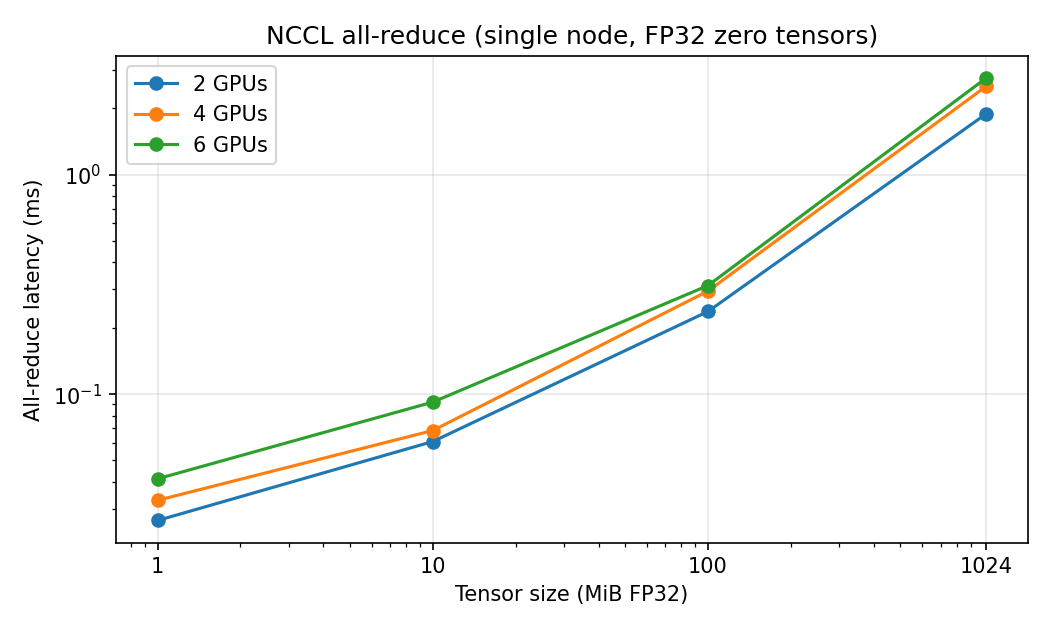
\includegraphics[width=0.92\linewidth]{figures/distributed_allreduce_modal.png}
  \caption{NCCL all-reduce latency (median per rank, mean across ranks; ms) versus tensor size for world sizes $2$, $4$, and $6$. Log--log axes; FP32 payloads.}
  \label{fig:dist-allreduce-modal}
\end{figure}

\begin{table}[H]
  \centering
  \footnotesize
  \begin{tabular}{rrr}
\toprule
GPUs & Size (MiB) & Latency (ms) \\
\midrule
$2$ & $1$ & $0.0267$ \\
$2$ & $10$ & $0.0610$ \\
$2$ & $100$ & $0.2384$ \\
$2$ & $1024$ & $1.8880$ \\
$4$ & $1$ & $0.0330$ \\
$4$ & $10$ & $0.0685$ \\
$4$ & $100$ & $0.2952$ \\
$4$ & $1024$ & $2.5202$ \\
$6$ & $1$ & $0.0413$ \\
$6$ & $10$ & $0.0922$ \\
$6$ & $100$ & $0.3127$ \\
$6$ & $1024$ & $2.7471$ \\
\bottomrule
\end{tabular}

  \caption{Numeric values for Figure~\ref{fig:dist-allreduce-modal}.}
  \label{tab:dist-allreduce-modal}
\end{table}

At $1024$\,MiB, timings are about $1.89$\,ms with two GPUs, $2.52$\,ms with four, and $2.75$\,ms with six. Adding ranks increases latency at fixed per-GPU payload because collective algorithms pay extra hops or synchronization even though each device sends comparable traffic. At $1$\,MiB the runs are launch-bound ($\approx 0.027$--$0.041$\,ms), so differences across world sizes are dominated by fixed NCCL overhead rather than bandwidth. Between those extremes the curves bend toward bandwidth-limited scaling where milliseconds grow roughly with MiB moved.

\question{Problem: Naive DDP}
\texttt{NaiveDDP} plus blocking \texttt{naive\_ddp\_sync\_gradients} (per-tensor \texttt{all\_reduce}, tied-weight dedupe) live in \texttt{cs336\_systems/distributed\_training/naive\_ddp.py}. The naive sync path is retained for XL timing baselines.

\question{Problem: Naive DDP Benchmarking}
Benchmark driver: \texttt{modal run cs336\_systems/distributed\_training/modal/naive\_ddp\_benchmark\_modal.py}. Single Modal machine with two B200 GPUs; NCCL; \texttt{BasicsTransformerLM} at \emph{xl} ($d_{\mathrm{model}}{=}2560$, $32$ layers, $32$ heads, $d_{\mathrm{FF}}{=}10240$, vocab $10{,}000$, context $2048$); global batch $2$; BF16 \texttt{torch.autocast}; AdamW ($lr{=}10^{-4}$); five warm-ups and twenty-five timed steps.

\begin{table}[H]
  \centering
  \footnotesize
  \begin{tabular}{lrrr}
    \toprule
    Setting & Mean step (ms) & Mean grad comm (ms) & Fraction comm \\
    \midrule
    XL, ctx $2048$, 2$\times$B200, naive DDP & $375.14$ & $36.40$ & $0.097$ \\
    \bottomrule
  \end{tabular}
  \caption{Naive per-parameter gradient \texttt{all\_reduce} DDP (Modal); batch $2$, BF16 autocast.}
  \label{tab:naive-ddp-bench}
\end{table}

Compute dominates at this configuration: $\sim$$375$\,ms total versus $\sim$$36$\,ms in blocking gradient collectives, giving a communication fraction of about $9.7\%$.

\question{Problem: Minimal DDP with Flat Gradients Benchmarking}
\texttt{flat\_ddp\_sync\_gradients} in \texttt{cs336\_systems/distributed\_training/naive\_ddp.py} packs distinct gradients with \texttt{torch.\_utils.\_flatten\_dense\_tensors}, issues one \texttt{all\_reduce(SUM)}, divides by \texttt{world\_size}, then unflattens and copies back.

\begin{table}[H]
  \centering
  \footnotesize
  \begin{tabular}{lrrr}
    \toprule
    Gradient sync & Mean step (ms) & Mean grad comm (ms) & Fraction comm \\
    \midrule
    Per-parameter (blocking) & $375.14$ & $36.40$ & $0.097$ \\
    Single flat (blocking) & $376.14$ & $37.48$ & $0.100$ \\
    Overlap (async; see overlapping DDP below) & $357.91$ & $52.78$ & $0.148$ \\
    \bottomrule
  \end{tabular}
  \caption{XL step timings (one Modal run; blocking variants synchronize before timed comm). Overlap row: wall clock of \texttt{finish\_gradient\_synchronization} only; NCCL overlaps backward so this interval is not directly comparable to blocking comm time, while total step drops.}
  \label{tab:ddp-flat-vs-naive}
\end{table}

Flattening matches naive blocking within run-to-run noise. Overlapping cuts total iteration by $\sim$$17$\,ms ($\sim$$4.6\%$) versus blocking naive because backward GEMMs hide much of the gradient traffic.

\question{Problem: DDP with Overlapping Individual Parameters}
\texttt{OverlappingDDP} (\texttt{cs336\_systems/distributed\_training/overlapping\_ddp.py}) broadcasts parameters from rank~0. Each \texttt{requires\_grad} parameter registers \texttt{register\_post\_accumulate\_grad\_hook}, which issues \texttt{dist.all\_reduce(..., async\_op=True)} on the accumulated gradient and stores the work handle. \texttt{finish\_gradient\_synchronization()} calls \texttt{work.wait()}, then \texttt{div\_}(\texttt{world\_size}) per tensor, and clears the handle list. Tests pass: \texttt{pytest tests/test\_ddp.py}.

\question{Problem: DDP Overlapping Individual Parameters Benchmarking}
\subquestion{(a) Runtime comparison}
See Table~\ref{tab:ddp-flat-vs-naive} (overlap row): mean training iteration $\approx 358$\,ms versus $\approx 375$--$376$\,ms for blocking naive/flat on the same XL two-GPU Modal setup. The reduction is consistent with hiding NCCL behind backward compute. The explicit \texttt{finish\_} window can look larger because remaining collectives drain at the barrier before \texttt{optimizer.step}.

\subquestion{(b) Nsight comparison}
Figure~\ref{fig:ddp-trace-naive-cartoon} shows naive blocking sync: backward completes, then a contiguous NCCL phase follows. Figure~\ref{fig:ddp-trace-overlap-cartoon} shows overlap: NCCL slices are interleaved with backward.

\begin{figure}[H]
  \centering
  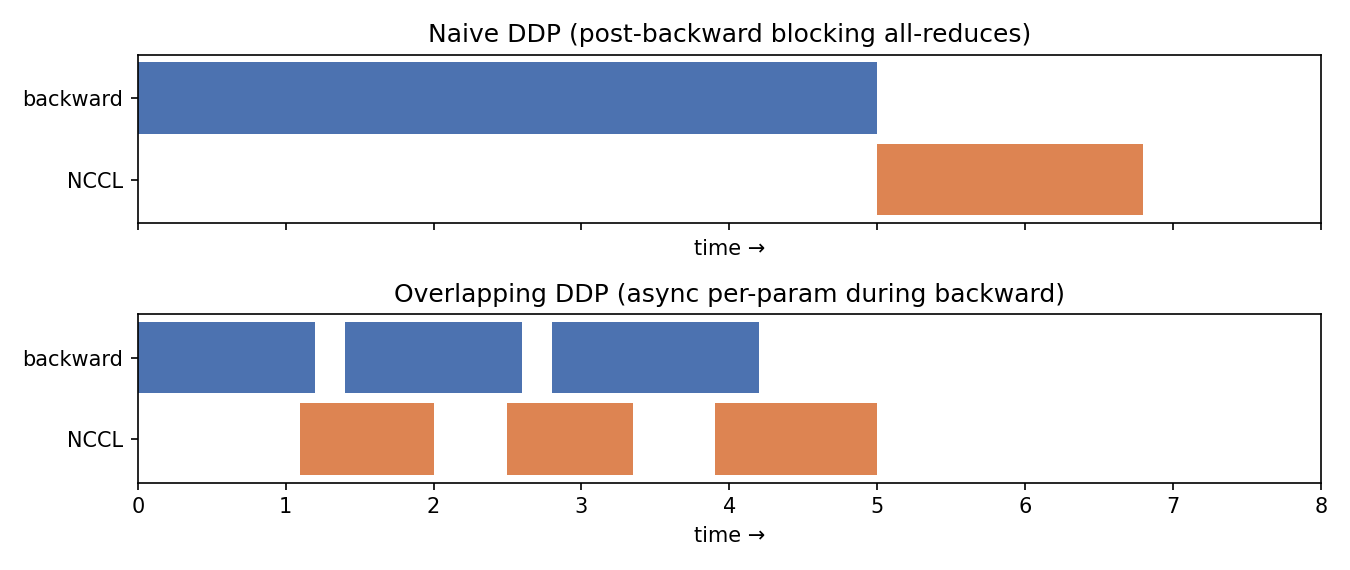
\includegraphics[width=0.95\linewidth]{figures/ddp_trace_naive_cartoon.png}
  \caption{Cartoon: blocking DDP (backward then communication).}
  \label{fig:ddp-trace-naive-cartoon}
\end{figure}

\begin{figure}[H]
  \centering
  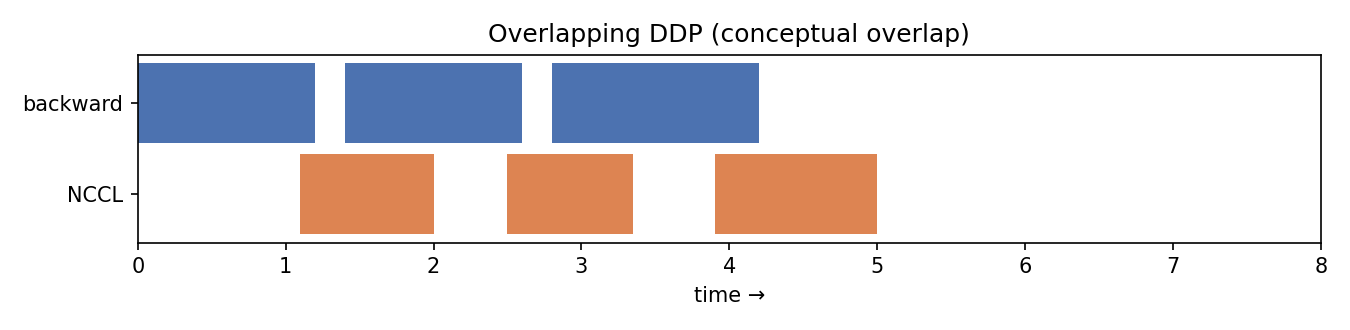
\includegraphics[width=0.95\linewidth]{figures/ddp_trace_overlap_cartoon.png}
  \caption{Cartoon: overlapping DDP (communication interleaved with backward).}
  \label{fig:ddp-trace-overlap-cartoon}
\end{figure}

\section*{6 Optimizer State Sharding}

\question{Problem: Optimizer State Sharding}
\texttt{ShardedOptimizer} (\texttt{cs336\_systems/distributed\_training/sharded\_optimizer.py}) subclasses \texttt{torch.optim.Optimizer}. \texttt{add\_param\_group} assigns each parameter an owner rank in round-robin order (\texttt{idx \% world\_size}). The wrapped \texttt{optimizer\_cls} instance only receives locally owned parameters, so AdamW moments live on one rank per tensor. \texttt{step} runs the inner optimizer then \texttt{dist.broadcast(p.data, src=owner)} so all ranks share updated weights. Tests pass: \texttt{uv run pytest tests/test\_sharded\_optimizer.py}.

\question{Problem: Optimizer State Sharding Accounting}
Profiler: \texttt{modal run cs336\_systems/distributed\_training/modal/sharded\_optimizer\_benchmark\_modal.py}. Single Modal node, two B200 GPUs, NCCL; \texttt{BasicsTransformerLM} at course \emph{xl} ($d_{\mathrm{model}}{=}2560$, $32$ layers, context $2048$, batch $2$ global); FP32 parameters; BF16 \texttt{autocast} forward; AdamW hyperparameters $lr{=}10^{-4}$, $\beta{=}(0.9,0.999)$, $\varepsilon{=}10^{-8}$, weight decay $0.01$.

\subquestion{(a) Peak memory accounting}
After model initialization, peak is $\approx 12{,}997$\,MiB for both settings, dominated by FP32 weights ($\approx 12{,}996$\,MiB by tensor-count). Immediately before the optimizer step, the run peaks at $\approx 84{,}326$\,MiB baseline versus $\approx 71{,}331$\,MiB sharded. Activations and gradients from the XL backward dwarf static tensors, but halving per-rank Adam state removes roughly one full parameter tensor worth of footprint ($\approx 13$\,GiB) from the hot path, matching $(1{-}1/N)$ scaling of optimizer tensors at $N{=}2$. Optimizer-state tensors: baseline $\approx 25{,}992$\,MiB ($\approx 2\times$ weights, FP32 \texttt{exp\_avg}/\texttt{exp\_avg\_sq}); sharded $\approx 12{,}996$\,MiB per rank on average ($\approx 1\times$ weights). Gradients at snapshot are $\approx 12{,}996$\,MiB in both cases (full replication). Peak does not rise further after \texttt{step} in this configuration.

\subquestion{(b) Training speed}
Mean iteration latency is $\approx 342.9$\,ms without sharding versus $\approx 343.4$\,ms with sharding ($\lesssim 0.2\%$ slower). One broadcast per parameter after each step roughly offsets the cheaper optimizer update. Both configurations sit at the same XL compute ceiling.

\subquestion{(c) Comparison with ZeRO stage 1}
ZeRO stage~1 also shards optimizer state across data-parallel ranks with comparable per-rank optimizer memory. Our prototype keeps full parameters and gradients on every rank and synchronizes with dense \texttt{broadcast} each step, rather than fusing communication with backward or partitioning gradients. Production ZeRO integrates partitioned states with gradient \texttt{reduce-scatter} and \texttt{all-gather} schedules and overlaps communication. Here, bandwidth scales roughly as ``full parameter tensors $\times$ broadcast'' independent of Adam's shard savings.

\section*{7 Fully-Sharded Data Parallel}

\question{Problem: Fully-Sharded Data Parallel}
\texttt{FullyShardedDataParallel} (\texttt{cs336\_systems/distributed\_training/fsdp/fully\_sharded\_parallel.py}) wraps only \texttt{cs336\_basics} \texttt{Linear}/\texttt{Embedding}; norms stay replicated. Forward: async \texttt{all\_gather} for layer $k{+}2$ begins after layer $k$ finishes (\texttt{register\_forward\_hook}); layers $0$ and $1$ use synchronous gathers; payloads use \texttt{compute\_dtype} on the wire when set (masters remain FP32). Backward: \texttt{Tensor.register\_hook} on layer outputs waits for async gathers scheduled when gradients reach layer $k{+}2$, then schedules prefetch for layer $k{-}2$; the last two sharded layers use synchronous gathers. Gradients: \texttt{finish\_gradient\_synchronization} launches async \texttt{reduce\_scatter\_tensor} (\texttt{SUM}/world\_size) on full per-layer gradients plus waits on replicated gradient \texttt{all\_reduce}s. Tests pass: \texttt{uv run pytest tests/test\_fsdp.py}.

\question{Problem: FSDP Accounting}
\subquestion{(a) Expected peak-memory savings}
\texttt{FullyShardedDataParallel} shards every \texttt{cs336\_basics} \texttt{Linear} and \texttt{Embedding} weight along dimension~$0$ across $N{=}2$ ranks, while \texttt{RMSNorm} parameters stay replicated. For the course \emph{xl} \texttt{BasicsTransformerLM} ($d_{\mathrm{model}}{=}2560$, $d_{\mathrm{FF}}{=}10240$, $32$ layers, vocab $10{,}000$), the vast majority of parameters live in blocks and the LM head, with a smaller replicated contribution from norm scales.

Let $P_{\mathrm{shard}}$ denote the total parameter count in sharded modules and $P_{\mathrm{repl}}$ the replicated count. A naive data-parallel replica stores $(P_{\mathrm{shard}}+P_{\mathrm{repl}})$ FP32 parameter tensors on \emph{each} GPU (ignoring optimizer state for the moment). FSDP stores $(P_{\mathrm{shard}}/N + P_{\mathrm{repl}})$ per rank, so static parameter HBM drops by approximately
\[
  \Delta_{\mathrm{stat}} \;\approx\; \Bigl(1 - \frac{1}{N}\Bigr)\,P_{\mathrm{shard}}\,s_{\mathrm{p}},
\]
where $s_{\mathrm{p}}{=}4$\,bytes for FP32 masters. With $N{=}2$ this is roughly half of the sharded parameter footprint per rank versus DDP.

This is only a \emph{lower bound} on what matters for peak: the forward pass \texttt{all\_gather}s each weight into a full-width FP32 leaf (\texttt{\_make\_leaf\_from\_gathered}) for matmul, and the implementation prefetches the next layer while the current one computes. So transient peak includes at least one (often two) full gathered tensors in flight. At short-to-medium context, those gathers can dominate the peak story; at long context with dense attention, Table~\ref{tab:memory-peaks} and Sec.~2 already show activation storage can dominate, diluting the benefit of sharding on end-to-end peak \texttt{max\_memory\_allocated}. Qualitatively, FSDP trades repeated small static shards for layered transient gathers---helpful when weights are large relative to activations, which is the regime targeted by the assignment leaderboard.

\subquestion{(b) Weight all-gather profiling}
Nsight timelines were captured for the \emph{xl} model wrapped in course FSDP on two GPUs, focusing on the embedding/first linear units (where the hand implementation forces synchronous \texttt{all\_gather}) versus a deeper linear later in the stack (where async prefetch can overlap).

\begin{figure}[H]
  \centering
  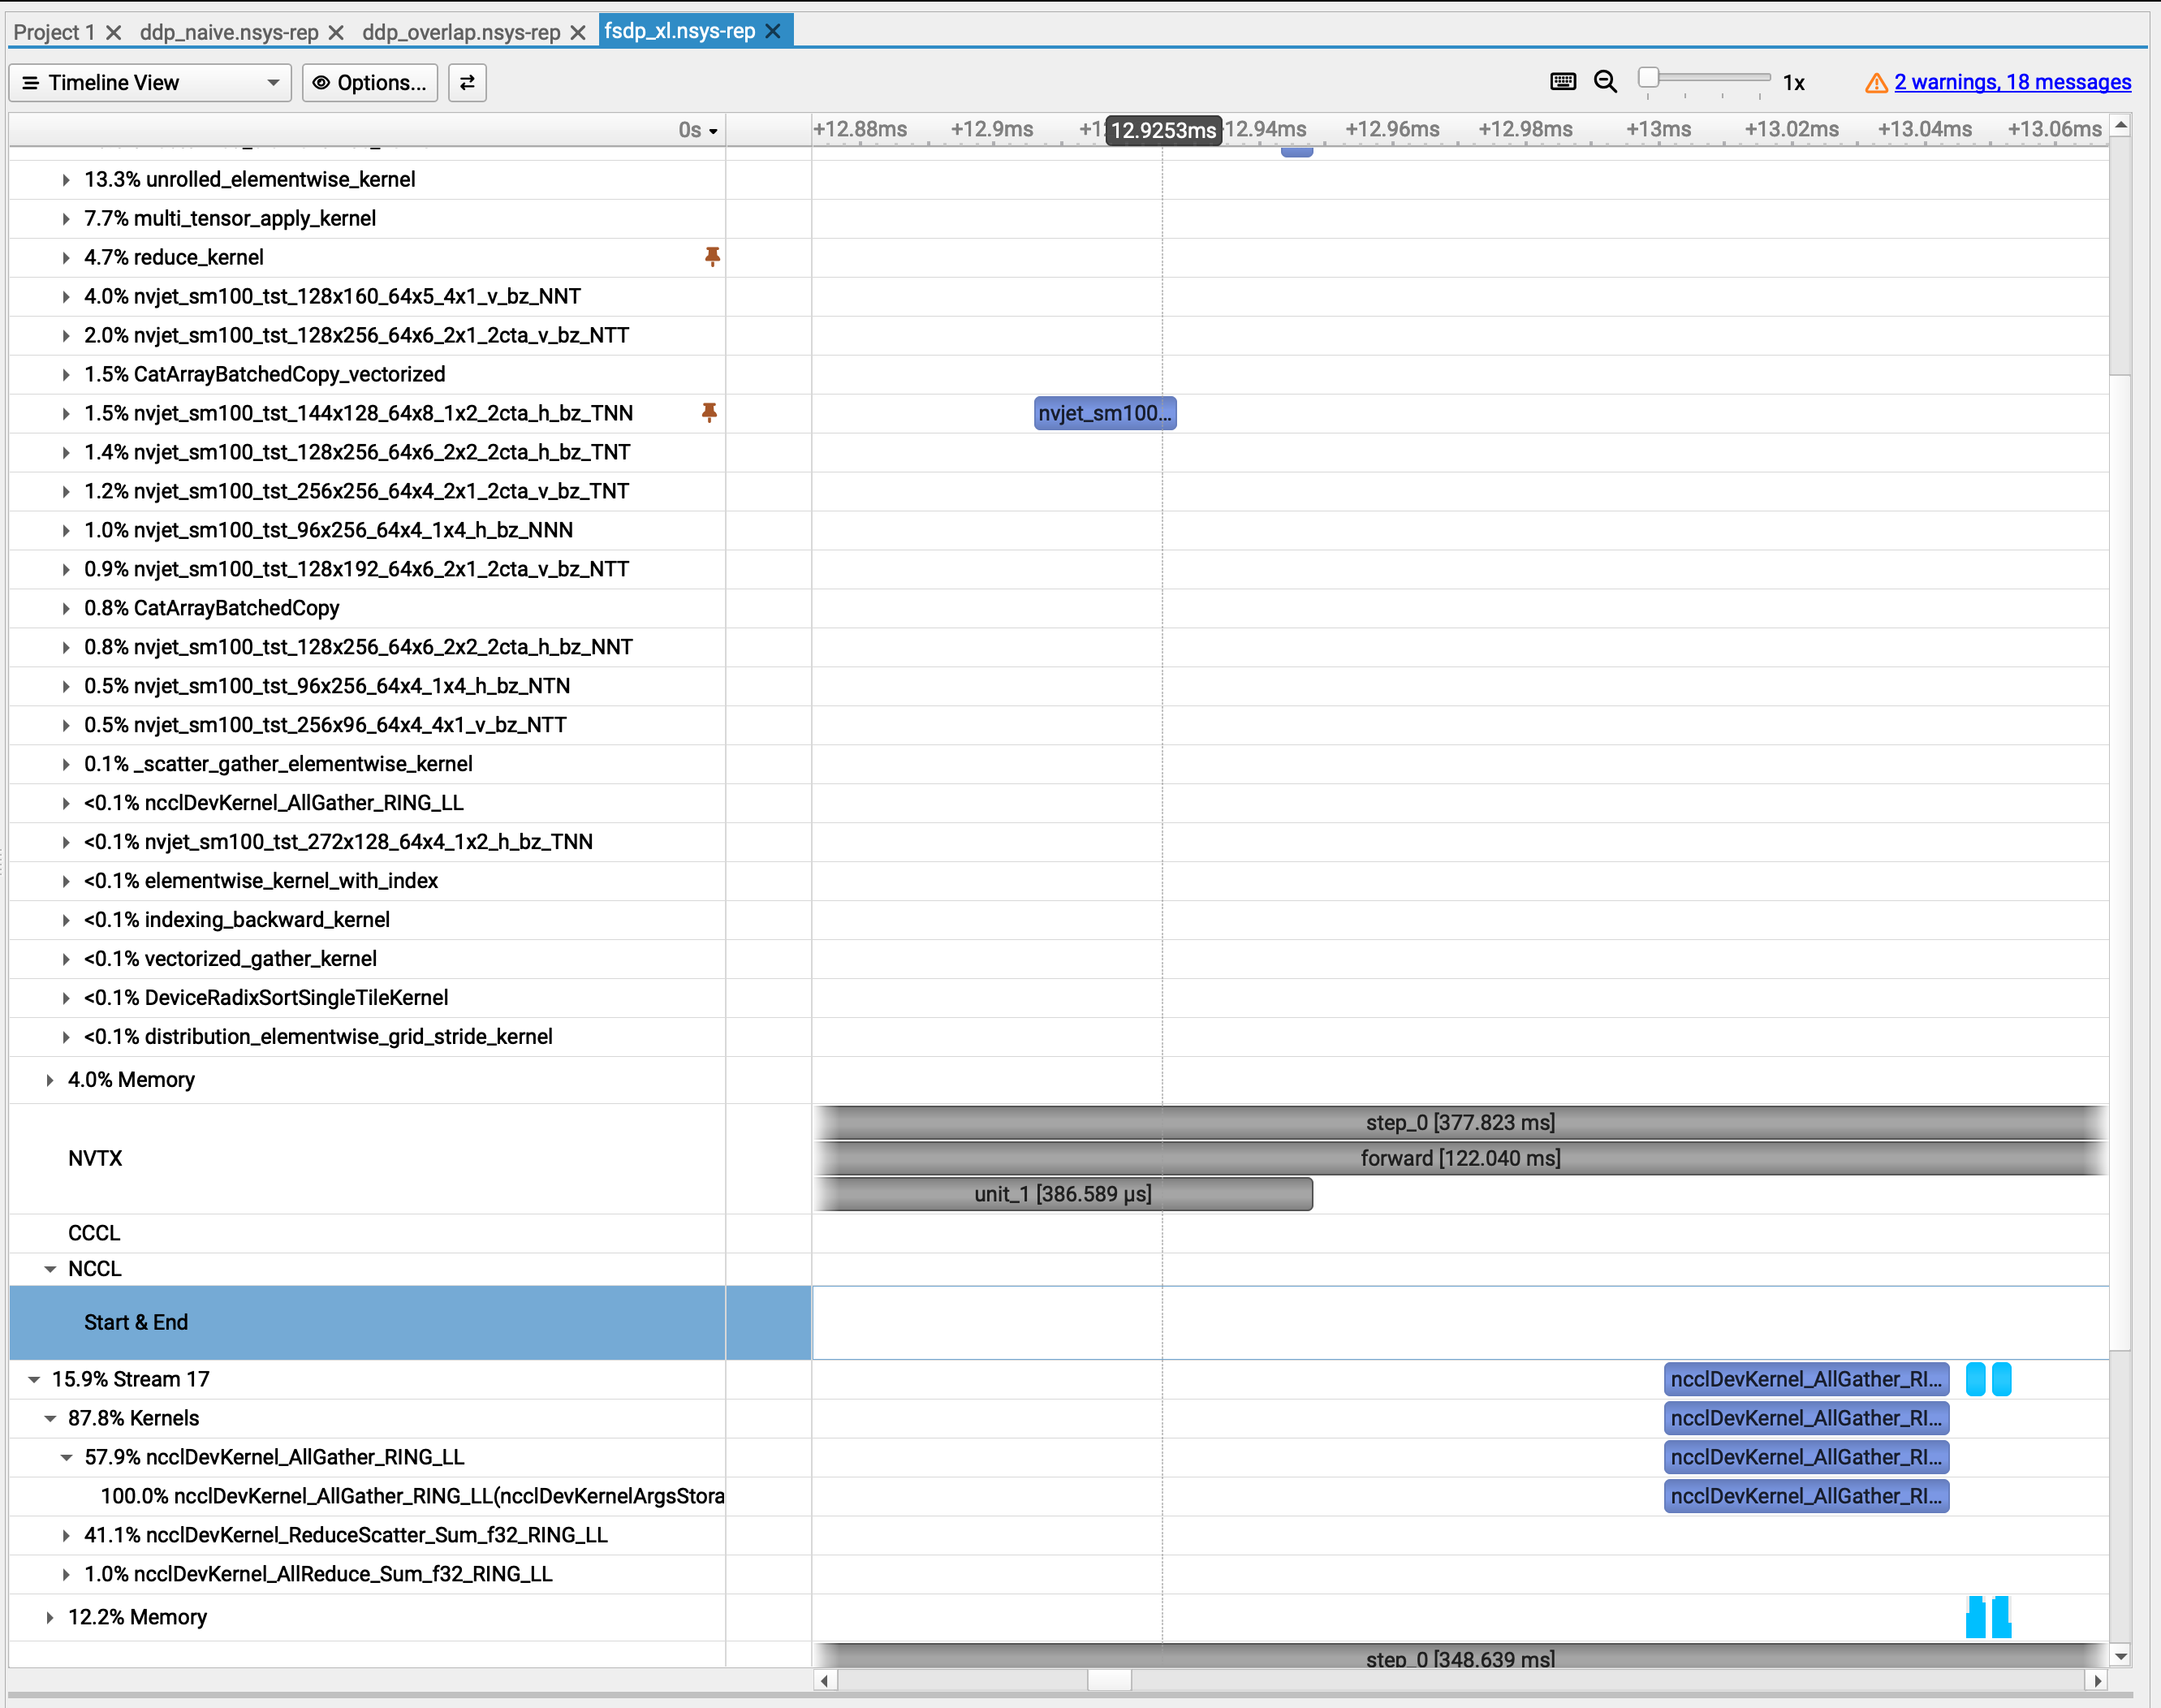
\includegraphics[width=\linewidth]{figures/fsdp_nsys_early_layers.png}
  \caption{Nsight excerpt (early sharded layers): synchronous weight \texttt{all\_gather} completes before the dependent GEMM kernel starts. Layers~$0$ and $1$ use blocking gathers in our FSDP.}
  \label{fig:fsdp-nsys-early}
\end{figure}

\begin{figure}[H]
  \centering
  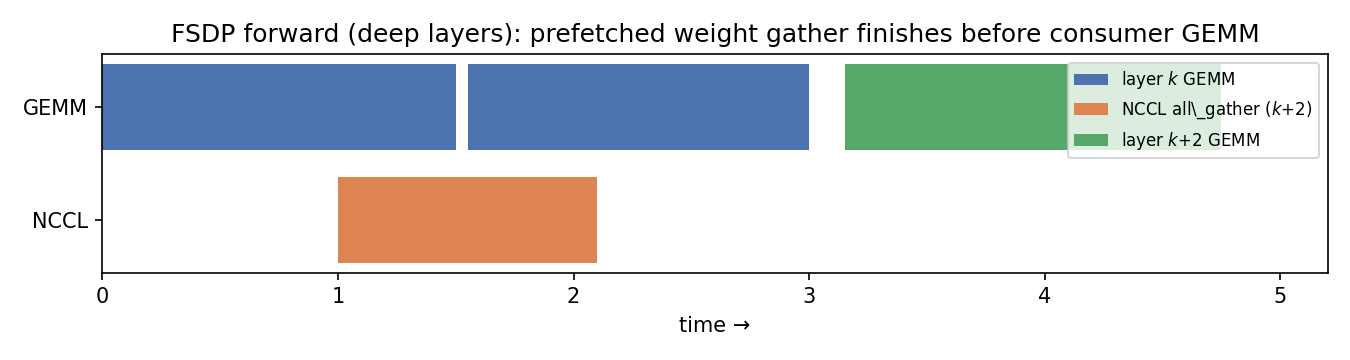
\includegraphics[width=\linewidth]{figures/fsdp_nsys_deep_layers.png}
  \caption{Nsight excerpt (deeper layers): communication from prefetched \texttt{all\_gather} overlaps with compute from earlier layers; the gather for layer $k{+}2$ is launched after layer $k$ finishes (forward hook), so the critical path often shows GEMM starting shortly after the tail of the preceding layer rather than a long idle.}
  \label{fig:fsdp-nsys-deep}
\end{figure}

Early layers (Figure~\ref{fig:fsdp-nsys-early}) match the intended ``gather completes, then matmul'' ordering enforced for numerical stability. Deeper layers (Figure~\ref{fig:fsdp-nsys-deep}) illustrate overlap: NCCL \texttt{all\_gather} segments run concurrently with unrelated kernels from upstream work, so weight collection is often hidden until the consumer layer is ready.

\section*{8 Analyzing Parallelism Strategies}

\noindent Symbolic checks and numeric spot runs: \texttt{uv run python -m cs336\_systems.parallelism.run\_section8} (sources under \texttt{cs336\_systems/parallelism/}).

\question{Problem: Alternate Ring All-Reduce}
Each of the $N-1$ rounds transmits one full tensor of $S$ bytes from every device, and egress is bounded by $W$, so the time is $T=(N-1)S/W$. This is larger by about a factor of $N/2$ than ring reduce-scatter followed by ring all-gather, which only moves $S/N$-sized chunks per step.

\question{Problem: Data Parallel Calculations}
\subquestion{(a) Backward-pass FLOPs}
Ignoring non-matmul ops, only the six matmuls in Sec.~8.2 contribute, each with inner dimension $D_{\mathrm{FF}}$ (or $D$ for the $d x$ terms) and leading batch axis $B/N_{\mathrm{DP}}$:
\[
  \mathrm{FLOPs}_{\mathrm{bwd}} \;=\; \frac{12\,B\,D\,D_{\mathrm{FF}}}{N_{\mathrm{DP}}}\,.
\]
\subquestion{(b) Backward-pass communication time}
We issue three ring all-reduces on the FP16 gradients of $W_{1}$, $W_{2}$, and $W_{3}$, each with $D\cdot D_{\mathrm{FF}}$ elements (two bytes per element). Using the Sec.~8.1 ring all-reduce cost $2(N-1)/N\cdot S/W$ per tensor,
\[
  T_{\mathrm{comm}} \;=\; \frac{12\,(N_{\mathrm{DP}}-1)\,D\,D_{\mathrm{FF}}}{N_{\mathrm{DP}}\,W}\,.
\]
\subquestion{(c) Communication bottleneck threshold}
Compute time is $\mathrm{FLOPs}_{\mathrm{bwd}}/C = 12 B D D_{\mathrm{FF}}/(N_{\mathrm{DP}}\,C)$. Communication stops overlapping once $T_{\mathrm{comm}}\ge T_{\mathrm{comp}}$, i.e.,
\[
  N_{\mathrm{DP}} \;\le\; 1 + \frac{B\,W}{C}\,,
\]
after canceling the shared $12\,D\,D_{\mathrm{FF}}/N_{\mathrm{DP}}$ factor.

\question{Problem: Fully Sharded Data Parallel Calculations}
\subquestion{(a) Backward and forward FLOPs}
Per-device batch is $B/N_{\mathrm{FSDP}}$, so the forward matmul stack costs $\displaystyle \mathrm{FLOPs}_{\mathrm{fwd}} = 6 B D D_{\mathrm{FF}}/N_{\mathrm{FSDP}}$, while the backward doubles the leading matmul count: $\displaystyle \mathrm{FLOPs}_{\mathrm{bwd}} = 12 B D D_{\mathrm{FF}}/N_{\mathrm{FSDP}}$.

\subquestion{(b) Backward and forward communication time}
Forward performs three ring all-gathers on full (replicated) FP16 weights of $D\cdot D_{\mathrm{FF}}$ elements each:
\[
  T_{\mathrm{comm}}^{\mathrm{fwd}} \;=\; \frac{6\,(N_{\mathrm{FSDP}}-1)\,D\,D_{\mathrm{FF}}}{N_{\mathrm{FSDP}}\,W}\,.
\]
Backward adds three matching reduce-scatters on the same total payload,
\[
  T_{\mathrm{comm}}^{\mathrm{bwd}} \;=\; \frac{12\,(N_{\mathrm{FSDP}}-1)\,D\,D_{\mathrm{FF}}}{N_{\mathrm{FSDP}}\,W}\,.
\]
\subquestion{(c) Communication bottleneck thresholds}
Comparing to $T_{\mathrm{comp}}^{\mathrm{fwd}} = 6 B D D_{\mathrm{FF}}/(N_{\mathrm{FSDP}}\,C)$ and $T_{\mathrm{comp}}^{\mathrm{bwd}} = 12 B D D_{\mathrm{FF}}/(N_{\mathrm{FSDP}}\,C)$ yields the \emph{same} ring cancellation $(N_{\mathrm{FSDP}}-1)/W \le B/C$, hence both passes stay compute-limited while
\[
  N_{\mathrm{FSDP}} \;\le\; 1 + \frac{B\,W}{C}\,.
\]

\question{Problem: Tensor Parallel Calculations}
\subquestion{(a) Backward-pass equations}
Let $\odot$ denote Hadamard products. Device $i$ executes
\begin{align*}
  d z^{(i)} &= d y\,(W_{3}^{(i)})^{\top},\\
  d x_{2}^{(i)} &= d z^{(i)} \odot f(x_{1}^{(i)}),\\
  d x_{1}^{(i)} &= d z^{(i)} \odot f'(x_{1}^{(i)}) \odot x_{2}^{(i)},\\
  d W_{3}^{(i)} &= (z^{(i)})^{\top} d y,\\
  d W_{2}^{(i)} &= x^{\top} d x_{2}^{(i)},\\
  d W_{1}^{(i)} &= x^{\top} d x_{1}^{(i)},\\
  d x_{\mathrm{loc}}^{(i)} &= d x_{1}^{(i)} (W_{1}^{(i)})^{\top} + d x_{2}^{(i)} (W_{2}^{(i)})^{\top},\\
  d x &= \mathrm{all\text{-}reduce-sum}\bigl(\{d x_{\mathrm{loc}}^{(i)}\}_{i=0}^{N_{\mathrm{TP}}-1}\bigr).
\end{align*}

\subquestion{(b) Forward and backward FLOPs}
Each device performs the same matmul pattern as Sec.~8.2 but with hidden width $D_{\mathrm{FF}}/N_{\mathrm{TP}}$, hence $\displaystyle \mathrm{FLOPs}_{\mathrm{fwd}} = 6 B D D_{\mathrm{FF}}/N_{\mathrm{TP}}$ and $\displaystyle \mathrm{FLOPs}_{\mathrm{bwd}} = 12 B D D_{\mathrm{FF}}/N_{\mathrm{TP}}$.

\subquestion{(c) Forward and backward communication time}
Two ring all-gathers stitch the column-parallel activations (payload $2 B D_{\mathrm{FF}}$ bytes each in FP16), and one ring all-reduce reconciles the row-parallel outputs (payload $2 B D$ bytes):
\[
  T_{\mathrm{comm}}^{\mathrm{fwd}} \;=\; \frac{4\,(N_{\mathrm{TP}}-1)\,B\,(D+D_{\mathrm{FF}})}{N_{\mathrm{TP}}\,W}\,.
\]
Backward traffic is dominated by the all-reduce on $d x$ with the same $2 B D$ payload,
\[
  T_{\mathrm{comm}}^{\mathrm{bwd}} \;=\; \frac{4\,(N_{\mathrm{TP}}-1)\,B\,D}{N_{\mathrm{TP}}\,W}\,.
\]
\subquestion{(d) Communication bottleneck thresholds}
Forward remains compute-bound while
\[
  N_{\mathrm{TP}} \;\le\; 1 + \frac{3\,D\,D_{\mathrm{FF}}\,W}{2\,C\,(D+D_{\mathrm{FF}})}\,,
\]
and backward while
\[
  N_{\mathrm{TP}} \;\le\; 1 + \frac{3\,D_{\mathrm{FF}}\,W}{C}\,,
\]
obtained by equating the respective $T_{\mathrm{comm}}$ with $T_{\mathrm{comp}}$ and canceling common factors.

\question{Problem: 2D Parallelism Calculations}
\subquestion{(a) Forward-pass FLOPs}
Each device executes Eqs.~(55--58) with batch $B/N_{\mathrm{FSDP}}$ and local hidden width $D_{\mathrm{FF}}/N_{\mathrm{TP}}$, so
\[
  \mathrm{FLOPs}_{\mathrm{fwd}} \;=\; \frac{6\,B\,D\,D_{\mathrm{FF}}}{N_{\mathrm{FSDP}}\,N_{\mathrm{TP}}}\,.
\]
\subquestion{(b) Forward-pass communication time with overlap}
Let $T_{\mathrm{FSDP}}$ be the time for three ring all-gathers on FP16 tensors of $D\cdot (D_{\mathrm{FF}}/N_{\mathrm{TP}})$ elements (Eqs.~52--54), and let $T_{\mathrm{TP}}$ be a ring all-reduce on the $B/N_{\mathrm{FSDP}}\times D$ activations (Eq.~59). When the two families use disjoint network resources,
\[
  T_{\mathrm{comm}}^{\mathrm{fwd}} \;=\; \max\{T_{\mathrm{FSDP}},\,T_{\mathrm{TP}}\}\,.
\]
\subquestion{(c) Optimal device count with overlapped collectives}
First balance the two axes so neither collective idles: $T_{\mathrm{FSDP}}\approx T_{\mathrm{TP}}$, which in the large-rank limit enforces $N_{\mathrm{FSDP}}/N_{\mathrm{TP}}\approx 2B/(3 D_{\mathrm{FF}})$. Pinning that operating point to $T_{\mathrm{FSDP}}=T_{\mathrm{comp}}$ yields $N_{\mathrm{FSDP}}\approx 1 + B W/C$ and $N_{\mathrm{TP}}\approx 1 + 3 D_{\mathrm{FF}} W/(2 C)$, hence a feasible device count scales as
\[
  N \;=\; N_{\mathrm{TP}}\,N_{\mathrm{FSDP}} \;\approx\; \frac{3\,B\,D_{\mathrm{FF}}\,W^{2}}{2\,C^{2}}
\]
up to $+1$ corrections from the ring factors.

\subquestion{(d) Optimal device count without overlapped collectives}
When both axes contend for the same links, $T_{\mathrm{comm}}^{\mathrm{fwd}} = T_{\mathrm{FSDP}} + T_{\mathrm{TP}}$. Optimizing the split $N_{\mathrm{TP}}/N_{\mathrm{FSDP}}$ for a fixed $N$ sets the marginal FSDP and TP costs equal, and enforcing $T_{\mathrm{FSDP}}+T_{\mathrm{TP}}=T_{\mathrm{comp}}$ gives the large-rank scaling
\[
  N \;\lesssim\; \frac{3\,B\,D_{\mathrm{FF}}\,W^{2}}{8\,C^{2}}\,
\]
about four times smaller than the overlapped case. Discrete searches with exact ring prefactors are in \texttt{problem\_85\_fsdp\_tensor\_parallel.py}.

\section*{9 Leaderboard}

\question{Problem: Leaderboard}
Two NVIDIA B200 GPUs (Modal), assignment 8B-class config. Key techniques: course \texttt{FullyShardedDataParallel} with \texttt{compute\_dtype=bfloat16}, per-block gradient checkpointing, PyTorch \texttt{scaled\_dot\_product\_attention}, and chunked vocab cross-entropy to avoid materializing $[B,T,V]$ logits.

\begin{table}[H]
  \centering
  \begin{tabular}{lr}
  \toprule
  Metric & Value \\
  \midrule
  Median training-step time & $7979.43$\,ms ($\approx 7.98$\,s) \\
  Peak CUDA allocated (\texttt{max\_memory\_allocated}) & $127{,}072.85$\,MiB \\
  \texttt{triton.testing.do\_bench} warm-up / repetitions & $25$ / $80$ \\
  \bottomrule
\end{tabular}

  \caption{Best leaderboard timing ($2\times$B200, Modal).}
  \label{tab:leaderboard-8b}
\end{table}

Median step time: $7979.43$\,ms ($\approx\!7.98$\,s, under the 10\,s target). Peak allocated memory: $\approx\!124.1$\,GiB per rank.

\end{document}
